\documentclass[final]{siamltex}
%\documentclass[12pt]{article}
\usepackage[dvips]{attachfile2}
\usepackage{mathdef}

\let\orightarrow\rightarrow
\let\omapsto\mapsto
\usepackage{breqn}
\let\rightarrow\orightarrow
\def\longrightarrow{\relbar\joinrel\joinrel\joinrel\orightarrow}
\let\mapsto\omapsto
\usepackage{hyperbreqn}

\def\be{\begin{dmath*}}
\def\ee{\end{dmath*}}
\def\bel{\begin{dmath}}
\def\eel{\end{dmath}}
\def\bec{\begin{dmath*}[compact]}
\let\eec\ee
\def\belc{\begin{equation}}
\def\eelc{\end{equation}}

\def\bg{\begin{dgroup*}}
\def\eg{\end{dgroup*}}
\def\bgl{\begin{dgroup}}
\def\egl{\end{dgroup}}
\def\bs{\begin{dsuspend}}
\def\es{\end{dsuspend}}
\def\no{\hiderel}

\newcommand{\Fourier}[0]{\mathcal{F}}

\begin{document}

%\title{Implicit Dealiasing of Fourier-Based Convolutions}
\title{Efficient Dealiased Convolutions without the Padding}
\author{John C. Bowman and Malcolm Roberts}
\maketitle

\begin{abstract}
An algorithm is described for dealiasing pseudospectral convolution sums
without the expense of conventional zero-padding or phase-shift
techniques. In the one-dimensional complex case, the memory requirements
are identical with the usual zero-padding technique, with the important
distinction that the additional work memory need not be contiguous with the
data. This decoupling of the data and work arrays significantly reduces the
memory usage of in-place higher-dimensional convolutions.
The technique also allows one to efficiently dealias the
hyperconvolutions that arise on Fourier transforming arbitrary powers.
Such implicitly padded convolutions can be built on top of state-of-the-art fast
Fourier transform libraries; for example, vectorized implementations of
multidimensional dealiased centered and non-centered, complex and Hermitian
convolutions, have already been implemented in the open-source package 
{\tt fftw++}. \end{abstract} 

\begin{keywords} 
dealiasing, convolution, zero padding, fast Fourier transform,
pseudospectral methods, spectral truncations, in-place Fourier transforms,
bit reversal, hyperconvolution
\end{keywords}

\begin{AMS}
65R99,65T50
%15A15, 15A09, 15A23
\end{AMS}

\pagestyle{myheadings}

%use out-of-place Fourier transforms where possible (percent?)

% decoupling is more convenient for the user, 
% 

%padding to smooth data vs. chirp-z algorithm

%vectorized with single-instruction multiple-data (SIMD) code.
%highly optimized

%avoids inconvenience of and extra copying required by zero padding

% CRAY power-of-2 stride issue
% Supports efficient convolutions of power of 2 sizes
%
% memory requirements of phase-shift \cite{Patterson and Orszag 71} (doubles
% memory usage).

% Think about parallelization issues (another advantage of removing zeros).

\section{Introduction}
Discrete convolution sums based on the fast Fourier transform (FFT) algorithm
have become important tools for image filtering, digital signal processing, and
correlation analysis. They are also widely used in computational physics to
solve nonlinear partial differential equations such as the Navier--Stokes
equations in periodic domains. In some of these applications, notably
direct numerical pseudospectral simulations of fluid turbulence, memory
usage is a critical limiting factor: in-place multidimensional Fourier
transforms are typically used to reduce the memory footprint of
the required spectral convolutions.

Because the discrete convolution, which produces cyclic output from cyclic
input, is applied to nonperiodic (wavenumber-space) data, it is important
to remove aliases from the convolution. Typically the data array is
extended by padding it with enough zeros so that the wave beats of the
the positive frequencies cannot wrap around and contaminate
the negative frequencies. The convolution is then performed using a
correspondingly larger Fourier transform size. Alternatively, phase
shift dealiasing \cite{Patterson71,Canuto} can be used to cancel out the
aliasing errors between two convolutions with two different phase
shifts. However, this second technique is rarely used in practice, since in
addition to doubling the memory requirements, it is computationally more
expensive ($15N\log_2 N$ operations) than zero padding
($\fr{45/4}N\log_2 N$ operations) \cite[p.~136]{Canuto}. 
% Address slightly misleading implication of Canuto page 136
% (dealiased.pdf: p.20) regarding power of 2 transforms (depends on
% application).

The obvious disadvantage of an explicit application of the zero padding
technique is that one is summing over a large number of data values that
are known {\it a priori\/} to be zero.
A frequently asked question by users of FFT libraries
who want to compute dealiased convolutions is how to avoid this obvious
waste of memory and computation time.
Steven G. Johnson, has provided this
answer\cite{http://www.fftw.org/pruned.html}:
\begin{quotation}
{\it
The most common case where people seem to want a pruned FFT is for
zero-padded convolutions, where roughly 50\% of your inputs are zero (to
get a linear convolution from an FFT-based cyclic convolution). Here, a
pruned FFT is hardly worth thinking about, at least in one dimension. In
higher dimensions, matters change (e.g. for a 3d zero-padded array about
1/8 of your inputs are non-zero, and one can fairly easily save a factor of
two or so simply by skipping 1d sub-transforms that are zero).
}
\end{quotation}

The reasoning behind the assertion that such one-dimensional pruned FFTs
are not worth thinking about is that if $K$ of the $N$ inputs are zero,
the computational cost is reduced only from $N\log N$ to $N\log K$.
For example, if $K=N/2$, the savings is a minuscule $1/\log_2 N$.
Nevertheless, in this work we demonstrate that pruning the zero-padded
elements of one-dimensional convolutions is indeed worth thinking about,
primarily because it provides a more effective building block for constructing
multidimensional convolutions.

The key observation is that, although the memory usage of our implicitly
padded 1D convolution is identical to that for a conventional explicitly
padded convolution, the additional temporary memory need not be contiguous
with the user data.  In a multidimensional context, this external work
buffer can be reused for other one-dimensional convolutions.
As a result, for dimensions greater than one, the memory usage of our
noncentered (centered) convolution is asymptotically one-half (two-thirds)
of the memory requirements imposed by zero padding.
Of course, if memory savings alone were the goal, this savings could
also be achieved with explicit zero padding by copying the data for the
innermost convolution to an external padded buffer, but such extra data
communication turns out to be prohibitively expensive. The fact that our
one-dimensional convolution does not require this extra copying is the key
feature that was exploited to obtain simultaneous improvements in memory
usage and performance.

The task of writing an efficient implicitly padded one-dimensional
convolution is onerous, particularly if one tries to compete with an
explicitly problem-dependent and architecture-adaptive FFTW algorithm such
as the award-winning \cite{FFTW} library, which empirically predetermines a
near optimal butterfly scheme at each subdivision. Effectively one wants to
perform the first FFT subdivision manually, dropping the zero terms and
leaving the inner transforms to be computed with the usual library
routine. But this places an artificial restriction, at least at the highest
subdivision, on the possible adaptive algorithm that can be
used. Fortunately, there are a number of features of our algorithm that
help to offset this disadvantage. First, since the goal is to produce a
convolution, bit-reversal for the manual (highest) subdivision is
unnecessary: the scrambled Fourier subtransforms of the two input vectors
can be multiplied together as they are produced (perhaps while are still
accessible in the cache). Second, the implicit method allows most (four out
of six for the complex noncentered case and seven out of nine for the
Hermitian centered case) of the subtransforms for an in-place convolution
to be computed as out-of-place transforms, which are typically faster than
in-place transforms.  These savings helped keep our one-dimensional in-place
implicit convolution competitive with the explicitly padded convolution
based on the same highly optimized library. 

The computation times for the two methods are compared for
one-dimensional noncentered (Fourier origin at the first index) complex
convolutions in Figure~\ref{timing1c} and one-dimensional centered (Fourier
origin at the central index) Hermitian convolutions in Figure~\ref{timing1r}.
Both the FFTW library and the layer we built on top of it were compiled
with the Intel C/C++ Compiler and optimization options and run on a 64-bit
Intel processor. 

For the noncentered case, where the origin is at the first index, the input
data vectors of length $m$ must each be zero-padded to length $n\ge 2m-1$ to
prevent the wavenumber $m-1$ from beating with itself to
affect mode~$n=0\mod n$. However, since power-of-two transforms are the most
efficient in practice, it is typically better to extend the padding to $n=2m$.

For the centered case, we take the input data length to be odd, say $2m-1$,
with the origin at index $m-1$. One then needs to pad to $n\ge 3m-2$
to prevent the wavenumber $m-1$ from beating with itself to affect the most
negative (first) wavenumber, $-m+1$. Asymptotically, for large $m$, this
argument yields the so-called $2/3$ padding rule. 
For implicit padding it is convenient to pad to $n=3m$ to allow use of a
radix $3$ subdivision at the highest level. For explicit padding, we chose
$n$ to be a power of $2$ and set FIXME$m$ to be the largest odd integer less than or
equal to $\ceil{(2n-1)/3}$, whereas for implicit padding, we chose $m$ itself
to be a power of $2$; thereby choosing the optimal size for each case
(for the intended application of solving partial differential equations,
the exact size is arbitrary anyway and is chosen in this manner to yield
optimal efficiency). 

%USE DISTINCT MONO MARKERS & LINE TYPES.
%With fftw-3.2.2 configured with --enable-sse2 and CC=icpc
\begin{figure}[htbp]
  \begin{center}
    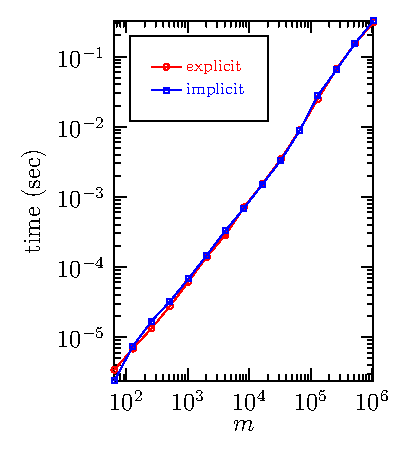
\includegraphics{timing1c}
    \caption{Comparison of computation times for explicitly and implicitly
dealiased complex noncentered 1D in-place convolutions of two vectors of
(unpadded) length $m$.}
    \label{timing1c}
  \end{center}
\end{figure}

\begin{figure}[htbp]
  \begin{center}
    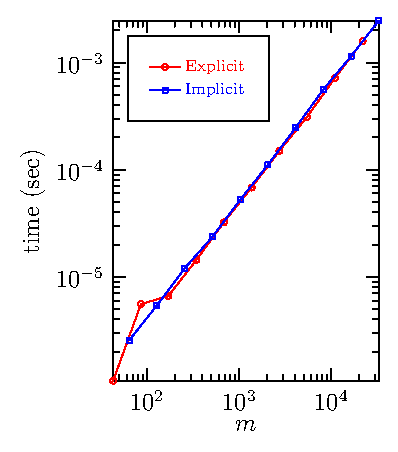
\includegraphics{timing1r}
    \caption{Comparison of computation times for explicitly and implicitly
dealiased Hermitian centered 1D in-place convolutions of two vectors of
(unpadded) length $2m-1$.}
    \label{timing1r}
  \end{center}
\end{figure}

\section{1-D Dealiased Fast Fourier Transforms}
\subsection{$1/2$ Dealiased Data}

Suppose $N$ is a multiple of $2$. 
In terms of the $N$th primitive root of unity,
$$
\zeta_N\doteq \exp\(\frac{2 \pi i}{N}\),
$$
the discrete inverse Fourier transform may be written
$$
u_j=\sum_{k=0}^{N-1}\zeta_N^{jk} \hat u_k\qquad j=0,\ldots,N-1.
$$
Notice that $\zeta_N^2=\zeta_{N/2}$ and $\zeta_N^N=1$.

If $\hat u_k=0$ for $k \ge N/2$ then
\be
u_{2\ell}
=\ds\sum_{k=0}^{N/2-1}\zeta_{N/2}^{\ell k} \hat u_k
%=\ds\sum_{m=0}^{N/4-1}\zeta_{N/2}^{2\ell m} \hat u_{2m}+
%\zeta_N^{2\ell}\sum_{m=0}^{N/4-1}\zeta_{N/2}^{2\ell m} \hat u_{2m+1}.
\ee

Likewise,
\be
u_{2\ell+1}
=\ds\sum_{k=0}^{N/2-1}\zeta_{N/2}^{\ell k} \zeta_N^k\hat u_k
%=\ds\sum_{m=0}^{N/4-1}\zeta_{N/2}^{2\ell m} \zeta_N^{2m}\hat u_{2m}
%+\zeta_N^{2\ell+1}\sum_{m=0}^{N/4-1}\zeta_{N/2}^{2\ell m} \zeta_N^{2m}\hat u_{2m+1}
\ee

These terms need to be computed for $\ell=0,\ldots,N/2-1$.
So the scaling is $2\fr{N}{2}\log {N/2}=N\log(N/2)$.


The odd and even terms of the convolution can be separately computed,
multiplied term-by-term, and transformed back to Fourier space:
\bec
\hat u_k=\sum_{j=0}^{N-1}\zeta_N^{-kj} u_j
=\sum_{\ell=0}^{N/2-1}\zeta_N^{-2k\ell} u_{2\ell}
+\zeta_N^{-k}\sum_{\ell=0}^{N/2-1}\zeta_N^{-2k\ell} u_{2\ell+1}
=\sum_{\ell=0}^{N/2-1}\zeta_{N/2}^{-k\ell} u_{2\ell}
+\zeta_N^{-k}\sum_{\ell=0}^{N/2-1}\zeta_{N/2}^{-k\ell} u_{2\ell+1}
\qquad k=0,\ldots,\fr{N}{2}-1.
\ee

We can therefore compute the convolution with two 1024 blocks (rather than one
2048 block), to get a dealiased 1024 convolution (with the 2/4 rule).

\newpage
\subsection{$2/3$ Dealiased Data}
The convolution in the Navier--Stokes equations require a $2/3$ padding in
order to avoid problems with aliasing.  Suppose that the total number of modes
(including zero-padding) is $N=3m$.  The inverse discrete Fourier transform
is then
$$
u_j=\sum_{k=0}^{N-1}\zeta_N^{jk} \hat u_k
=\sum_{k=0}^{2m-1}\zeta_N^{jk} \hat u_k
$$
Then 
\bel
u_{3\ell}= \sum_{k=0}^{2m-1}\z_{3m}^{3\ell k} \hat u_k
=\sum_{k=0}^{m-1}\z_{m}^{\ell k} \hat u_k
+\sum_{k=m}^{2m-1}\z_{m}^{\ell k} \hat u_k
=\sum_{k=0}^{m-1}\z_{m}^{\ell k} \hat u_k
+\sum_{k=0}^{m-1}\z_{m}^{\ell (k+m)} \hat u_{k+m}
=\sum_{k=0}^{m-1}\z_{m}^{\ell k} \(\hat u_k+\hat u_{k+m}\).\label{DFTm}
\eel
Equation~\ref{DFTm} is a DFT of length $m$,
each requiring $m\log m$ operations. Following a similar procedure,
with $r=1$ or $r=2$,
\bel
\label{dfft23g}
u_{3\ell +r}\no=
 \sum_{k=0}^{m-1}\z_{m}^{\ell k} \(\z_N^{rk} \hat u_k + \z_N^{r(k+m)}\hat u_{k+m}\)
\eel
Thus, the total number of operations is $3 m \log m = N \log\frac{N}{3}$.

The forward Fourier transform appears as
\be
\hat u_k=\sum_{j=0}^{N-1}\zeta_N^{-kj} u_j
=\sum_{r=0}^{2}\zeta_N^{-rk}\sum_{\ell=0}^{m-1}\zeta_N^{-3\ell k} u_{3\ell+r}
=\sum_{r=0}^{2}\zeta_N^{-rk}\sum_{\ell=0}^{m-1}\zeta_m^{-\ell k} u_{3\ell+r}
\qquad k\no =0,\ldots,pm-1.
\ee

\newpage
\subsubsection{1D Complex to Real Transforms of 2/3 Dealiased Data}

Consider the cryptic comment
\begin{quotation}
  ``Also, this will work with complex to real transforms without modification,
  since $\zeta_N^{-k}=\zeta_N^k{}^*$.''
\end{quotation}
As it turns out, $2/3$ dealiased data works particularly well with the
Hermiticity condition, $\hat{u}_{-k}=\hat{u}^*_k$, which guarantees
that the $x$-space data is real-valued. Consider a
wavenumber-truncated vector ranging from $k=-(m-1)$ to $k=m-1$, which
has $2m-1$ elements.

The backwards (complex-to-real) transform becomes, on letting $k'=m+k$,
\bec
u_{3\ell +r}\no=\sum_{k=-m+1}^{m-1}\z_{m}^{\ell k} \z_N^{rk} \hat u_k
=\sum_{k'=1}^{m-1}\z_{m}^{\ell k'} \z_N^{r(k'-m)} \hat u_{k'-m}
+\sum_{k=0}^{m-1}\z_{m}^{\ell k} \z_N^{rk} \hat u_k
=\sum_{k=1}^{m-1}\z_{m}^{\ell k} \z_N^{-r(m-k)} \hat u_{m-k}^*
+\sum_{k=0}^{m-1}\z_{m}^{\ell k} \z_N^{rk} \hat u_k
=\sum_{k=0}^{m-1}\z_{m}^{\ell k} \(w_{k,r}+w_{m-k,r}^*\),
\ee
where
$$
w_{k,r}=\z_N^{rk} \(\hat u_k-\half \hat u_0\d_{k,0}\).
$$
The forwards transform becomes
\be
\hat u_k=\sum_{j=0}^{N-1}\zeta_N^{-kj} u_j
=\sum_{r=-1}^{1}\zeta_N^{-rk}\sum_{\ell=0}^{m-1}\zeta_N^{-3\ell k} u_{3\ell+r}
=\sum_{r=-1}^{1}\zeta_N^{-rk}\sum_{\ell=0}^{m-1}\zeta_m^{-\ell k} u_{3\ell+r}
\qquad k\no =0,\ldots,m-1.
\ee

Note: without the hermiticity condition, the backwards transform is
\bec
u_{3\ell +r}\no=\sum_{k=-m+1}^{m-1}\z_{m}^{\ell k} \z_N^{rk} \hat u_k
=\sum_{k'=1}^{m-1}\z_{m}^{\ell k'} \z_N^{r(k'-m)} \hat u_{k'-m}
+\sum_{k=0}^{m-1}\z_{m}^{\ell k} \z_N^{rk} \hat u_k
=\sum_{k=0}^{m-1}\z_{m}^{\ell k} w_{k,r},
\ee
where
$$
w_{k,r}=
\cases{
\hat u_0&if $k=0$,\cr
\z_N^{rk}(\hat u_k+\z_3^{-r}\hat u_{k-m})&if $1\le k\le m-1$.\cr
}
$$
and the forwards transform is
\be
\hat u_k=\sum_{j=0}^{N-1}\zeta_N^{-kj} u_j
=\sum_{r=-1}^{1}\zeta_N^{-rk}\sum_{\ell=0}^{m-1}\zeta_m^{-\ell k} u_{3\ell+r}
\qquad k\no =-m+1,\ldots,m-1.
\ee



\subsubsection{2D Complex to Real Transforms of 2/3 Dealiased Data}
The Hermiticity condition is now $\hat{u}_{-k,-\ell}=\hat{u}^*_{k,\ell}$.
The procedure is analagous as in 1D,
where we interpret each index as a vector, add dot products,
split the two-dimensional sum into lower and upper halves, and use the
change of variables $\vk=(m_x,m_y)+\vk'$.
\begin{comment}
\bec
u_{3u+r,3v+s}\no=\sum_{k=-m-1}^{m-1}\sum_{\ell=-m-1}^{m-1}
\z_{m}^{u k} \z_{m}^{v \ell} \z_N^{rk} \z_N^{s\ell} \hat u_{k,\ell}
=\sum_{k=-m-1}^{m-1}\z_{m}^{u k}\z_N^{rk}  
\sum_{\ell=1}^{m-1} \z_{m}^{v \ell} \z_N^{s(\ell'-m)} \hat u_{k,\ell'-m}
+\sum_{k=-m-1}^{m-1}\z_{m}^{u k}\z_N^{rk}
\sum_{\ell=0}^{m-1} \z_{m}^{v \ell} \z_N^{s\ell} \hat u_{k,\ell}
=\sum_{k=-m-1}^{m-1}\z_{m}^{-u k}\z_N^{-rk}  
\sum_{\ell=1}^{m-1} \z_{m}^{v \ell} \z_N^{-s(m-\ell')} \hat u_{k,m-\ell'}^*
+\sum_{k=-m-1}^{m-1}\z_{m}^{u k}\z_N^{rk}
\sum_{\ell=0}^{m-1} \z_{m}^{v \ell} \z_N^{s\ell} \hat u_{k,\ell}
\ee
\end{comment}


\newpage
\subsection{$p/q$ Dealiased Data}

In general, consider a ``$p/q$'' padding in which $N=qm$, and only $pm$ modes
are non-zero, with $p$ and $q$ relatively prime. Consider $u_{q\ell+r}$, with
$\ell=0 \dots m-1$, $r=0 \dots q-1$.
Then
\be
u_{q\ell+r} = \sum_{k=0}^{N-1}\z_N^{(q\ell+r)k} \hat u_k
= \sum_{k=0}^{pm-1}\z_{qm}^{(q\ell+r)k} \hat u_k
= \sum_{k=0}^{pm-1}\z_{m}^{\ell k}\z_{N}^{rk} \hat u_k
= \sum_{\a=0}^{p-1} \sum_{k=\a m}^{(\a+1)m-1}\z_{m}^{\ell k}\z_{N}^{rk} \hat u_k
= \sum_{\a=0}^{p-1} \sum_{\k=0}^{m-1}\z_{m}^{\ell (\k+\a m)}\z_{N}^{r(\k+\a m)}
\hat u_{\k+\a m}
%=  \sum_{\a=0}^{p-1}\z_N^{r \a m} \sum_{\k=0}^{m-1}\z_m^{\ell\k}\z_N^{r\k}\hat u_{\k+\a m}
=  \sum_{\k=0}^{m-1}\z_m^{\ell\k}\sum_{\a=0}^{p-1}\z_N^{r(\k+\a m)} \hat u_{\k+\a m}
\ee .
Note that, in the last line, we have the choice of which $\z$ to use, since
$\z_q^{r \a}=\z_N^{r \a m}$. Since there are $m$ choices of $r$ and $q$ choices
for $\ell$, we are left with $mq=N$ FFTs of length $p$, leaving on the order
of $N \log p = N \log (N/q)$ operations.  Again, while the computational
savings is only marginal, this formulation affords signficant improvements
in memory use and parallelizability.

The forward Fourier transform appears as
\be
\hat u_k=\sum_{j=0}^{N-1}\zeta_N^{-kj} u_j
=\sum_{r=0}^{q-1}\zeta_N^{-rk}\sum_{\ell=0}^{m-1}\zeta_N^{-q\ell k} u_{q\ell+r}
=\sum_{r=0}^{q-1}\zeta_N^{-rk}\sum_{\ell=0}^{m-1}\zeta_m^{-\ell k} u_{q\ell+r}
\qquad k\no =0,\ldots,pm-1.
\ee

%TODO: I think that this can be generalized in the following fashion:
%if $m$ of the $N$ modes are non-zero, let $p=N/\gcd(m,N)$. Then we
%have can divide up the DFT into $p$ DFTs of length $m$. Must work out
%the details.




\section{2D, 2/3-dealiased transforms}
Our goal is to apply this to dealiased pseudospectral simulations. If we 
avoid moving the $k$-space origin to the middle of the array, the Fourier
data is sparse, with a square of length $2/3$ being non-zero. Suppose that 
the first FFT is done in the $x$ direction.  Then, $1/3$ of the transforms
are zero, and can be ignored. The remaining transforms are $2/3$ dealiased,
each of which can be done with $n \log (2 n/3)$ operations. This leaves
the upper $1/3$ modes set to zero.  The final transform, done in the 
$y$-direction, takes $n \log(2 n/3)$ operations.  See figure \ref{dealias2d}.
The total cost is then
\be
\frac{2 n}{3} \log \frac{2 n}{3} +  n \log \frac{2 n}{3}
=\frac{5n}{3} \log \frac{2 n}{3},
\ee
using the dealiased FFT, as opposed to $2 n \log n$ for the naive FFT. This 
is $1/6$ faster, while using significantly less memory. Moreover, the
intermediary, $1/3$-sparse buffer can be kept allocated as an intermediary
buffer for all necessary transformations.
\begin{figure}[htbp]
  \begin{center}
    \includegraphics{dealias2d}
    \caption{Procedure for transforming 2D dealiased arrays.}
    \label{dealias2d}
  \end{center}
\end{figure}

\section{Conclusions}
In this work we develop an efficient method for avoiding explicit zero
padding in multidimensional convolutions, saving both memory and
computation time.

\end{document}

%Self-sorting in-place fast fourier transforms
%Source 	SIAM Journal on Scientific and Statistical Computing archive
%Volume 12 ,  Issue 4  (July 1991) table of contents
%Pages: 808 - 823  
%Year of Publication: 1991
%ISSN:0196-5204 

% LocalWords:  dealiasing dealias hyperconvolutions Hermitian fftw FFT priori
% LocalWords:  hyperconvolution nonperiodic FFTs noncentered subtransforms
% LocalWords:  unpadded
